\documentclass{beamer}
\usepackage{color, graphicx}
\usepackage{amsmath,amssymb}
\usepackage{wrapfig}
\usepackage[utf8]{inputenc}
\usecolortheme{crane}
%$\setbeamercovered{dynamic}
\setbeamertemplate{items}[circle]
\setbeamertemplate{blocks}[rounded][shadow=false]
\setbeamertemplate{navigation symbols}{}
\setbeamertemplate{footline}[frame number]{}

\title{Algorithmic Analysis\\ of Code-Breaking Games}
\author{\textbf{Miroslav Klimoš} \\\medskip Advisor: prof. RNDr. Antonín Kučera Ph.D.}

\date{June 2014}

\begin{document}

\begin{frame}[plain]
\begin{center}

\includegraphics[width=20mm]{logo_fi.pdf}
\end{center}
\vspace{-5mm}
\maketitle
\end{frame}

\begin{frame}{Code-breaking games}
\begin{itemize}
\item 2 players: \emph{codemaker + codebreaker}
\item codemakers selects a \emph{secret code}
\item codebreaker strives to reveal the code through \emph{experiments}
\item for each experiment, codemaker releases some \emph{partial information} about the code
\end{itemize}
\end{frame}

\begin{frame}{Mastermind}
\begin{columns}
 \begin{column}{.35\textwidth}
 \centering
 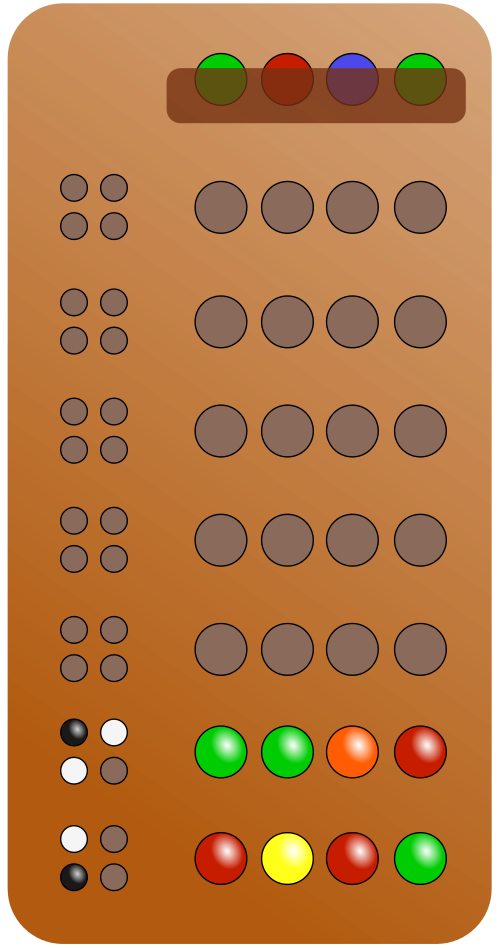
\includegraphics[width=3cm]{../pictures/mastermind.png}
 \end{column}

 \begin{column}{.6\textwidth}
  \begin{itemize}
  \item Code: 4 pegs $\times$ 6 colours
  \item Experiment $=$ guess
  % \item Evaluation with black and white markers\\
  \end{itemize}
  \begin{center}
  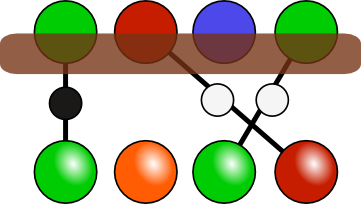
\includegraphics[width=3cm]{../pictures/mastermind-matching.png}
  \end{center}
 \end{column}
\end{columns}
\end{frame}

\begin{frame}{Challenges}
\begin{itemize}
\item Formal model of code-breaking games
% \item Strategies for experiment selection
\item Method for symmetry detection
\item Algorithms for strategy evaluation and synthesis
\item Computer language for game specification
\item Implementation of proposed algorithms
\end{itemize}
\end{frame}

\begin{frame}{Formal model}
\begin{itemize}
\item Game description
\begin{itemize}
\item set of propositional variables $X$
\item initial constraint $\varphi$
\item set of \emph{experiments} $E$
\end{itemize}

\item Secret code: valuation of $X$ (satisfying $\varphi$)
\item Partial information: formula in $X$
\item Strategy (memory-less): function $\textsc{form}_X \rightarrow E$
\end{itemize}
\end{frame}

\begin{frame}{Example}
\end{frame}

\begin{frame}{Symmetry detection}
\end{frame}

\begin{frame}{Strategies and algorithms}
\end{frame}

\begin{frame}{Game specification language}
\end{frame}

\begin{frame}{Implementation}
\end{frame}

\begin{frame}{Conclusions}
\end{frame}

\end{document}


